\documentclass[12pt,a4paper]{article}
\usepackage[utf8]{inputenc}
\usepackage{babel}
\usepackage{graphicx}
\usepackage{hyperref}
\usepackage{listings}
\usepackage{xcolor}
\usepackage{geometry}
\usepackage{tikz}
\usetikzlibrary{shapes,arrows,positioning,calc,fit}

\geometry{margin=1in}

\lstset{
    basicstyle=\ttfamily\small,
    breaklines=true,
    frame=single,
    backgroundcolor=\color{gray!5},
    keywordstyle=\color{blue},
    commentstyle=\color{green!60!black},
    stringstyle=\color{orange}
}

\title{Documentație Tehnică Completă: Unemployment Data Visualizer}
\author{Bazon Bogdan \\ Meraru Ioan-Lucian}
\date{\today}

\begin{document}

\maketitle
\tableofcontents
\newpage 

\section{Problem Definition}
Acest proiect presupune dezvoltarea unei aplicații web ce afișează datele despre șomajul în România prin anumite criterii (Rata de Șomaj, Mediul de proveniență, Vârstă, Nivel de Educație, etc.) și o anumită dată. Datele sunt preluate din \textbf{data.gov.ro} și aplicația are posibilitatea de a compara datele dintr-o anumită perioadă cu alta. Aplicația permite exportul de date prin CSV și PDF plus exportul grafurilor în SVG. De asemenea, aplicația dispune și de un sistem de caching pentru îmbunătățirea preluării datelor.

\section{Use Case Scenario}

\subsection{Use Case Diagram}
\begin{center}
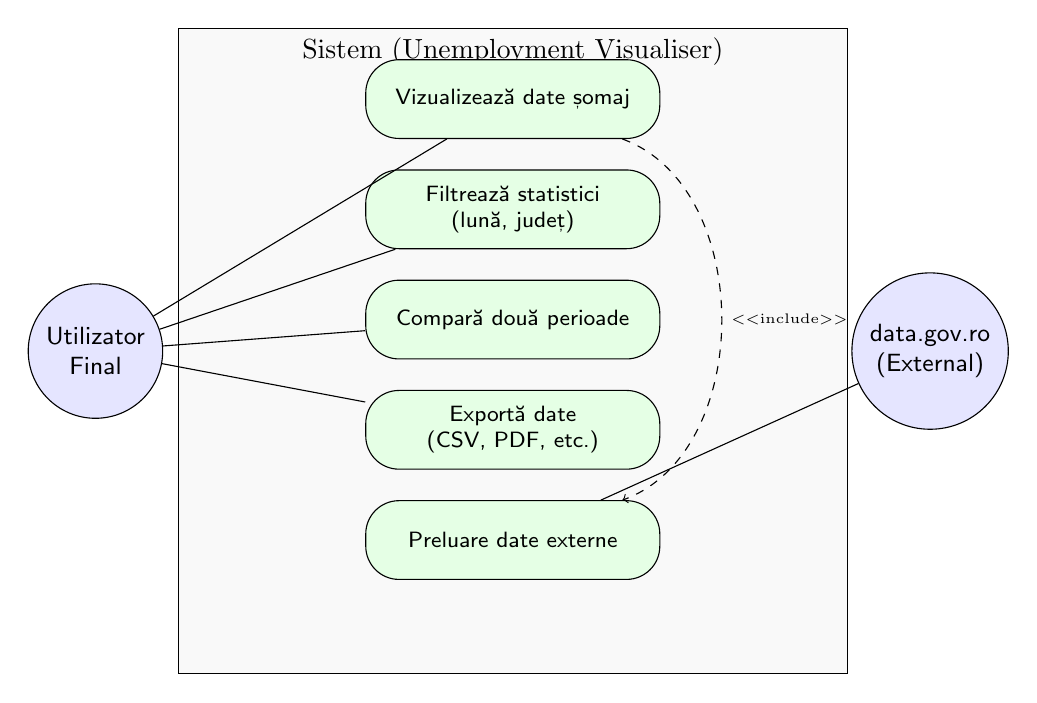
\begin{tikzpicture}[
    actor/.style={circle, draw, fill=blue!10, minimum size=1.2cm, font=\small\sffamily, align=center},
    usecase/.style={rectangle, draw, rounded corners=12pt, fill=green!10, text width=3.5cm, align=center, minimum height=1cm, font=\footnotesize\sffamily},
    system/.style={rectangle, draw, fill=gray!5, minimum width=8.5cm, minimum height=8.2cm, label={[shift={(0,-0.6)}]above:Sistem (Unemployment Visualiser)}}
]
    % Draw System Boundary
    \node[system] (sys) at (3.5, -2.0) {};

    % Actors
    \node[actor] (user) at (-1.8, -2.0) {Utilizator\\Final};
    \node[actor] (api) at (8.8, -2.0) {data.gov.ro\\(External)};

    % Use Cases
    \node[usecase] (uc1) at (3.5, 1.2) {Vizualizează date șomaj};
    \node[usecase] (uc2) at (3.5, -0.2) {Filtrează statistici (lună, județ)};
    \node[usecase] (uc3) at (3.5, -1.6) {Compară două perioade};
    \node[usecase] (uc4) at (3.5, -3.0) {Exportă date (CSV, PDF, etc.)};
    \node[usecase] (uc5) at (3.5, -4.4) {Preluare date externe};

    % Connections
    \draw (user) -- (uc1);
    \draw (user) -- (uc2);
    \draw (user) -- (uc3);
    \draw (user) -- (uc4);
    \draw (uc5) -- (api);
    
    % Include relation
    \draw[->, dashed] (uc1) to [bend left=70] node[right, font=\tiny] {<<include>>} (uc5);
\end{tikzpicture}
\end{center}

\subsection{Fluxul Principal}
Utilizatorul accesează platforma pentru a analiza evoluția șomajului. Poate filtra datele după lună, județ sau criteriu (vârstă, educație, mediu). Sistemul permite compararea a două perioade diferite pentru a observa tendințele economice.

\subsection{Gestionarea Erorilor (Ce se întâmplă dacă ceva nu merge bine)}
\begin{itemize}
    \item \textbf{Sursa externă indisponibilă}: Dacă \texttt{data.gov.ro} nu răspunde la cererea cURL, sistemul API returnează un cod HTTP 502 (Bad Gateway). Frontend-ul captează eroarea și afișează un mesaj de avertizare utilizatorului: „Nu s-au putut încărca datele. Verificați sursa externă.”
    \item \textbf{Date corupte în cache}: Dacă un fișier CSV descărcat este invalid, parserul backend va arunca o excepție. Utilizatorul poate forța reîmprospătarea prin ștergerea cache-ului din interfața de administrare/debug a API-ului.
    \item \textbf{Eroare de memorie la export}: Din cauza volumului mare de date, exportul PDF poate eșua în browsere cu memorie limitată. Sistemul folosește compresie JPEG pentru grafice și procesare asincronă pentru a minimiza acest risc.
\end{itemize}

\section{Diagrams (C4 Model)}

\subsection{Level 1: System Context Diagram}
\begin{center}
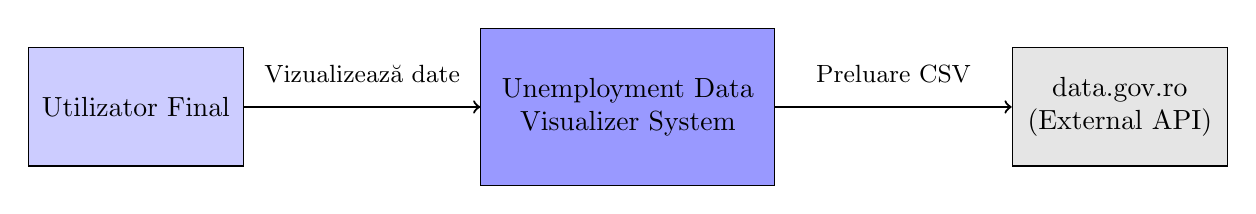
\begin{tikzpicture}[node distance=2cm, auto]
    \node[rectangle, draw, fill=blue!20, text width=2.5cm, align=center, minimum height=1.5cm] (user) {Utilizator Final};
    \node[rectangle, draw, fill=blue!40, text width=3.5cm, align=center, minimum height=2cm, right=3cm of user] (system) {Unemployment Data Visualizer System};
    \node[rectangle, draw, fill=gray!20, text width=2.5cm, align=center, minimum height=1.5cm, right=3cm of system] (datagov) {data.gov.ro (External API)};

    \draw[->, thick] (user) -- node[above=5pt, font=\small] {Vizualizează date} (system);
    \draw[->, thick] (system) -- node[above=5pt, font=\small] {Preluare CSV} (datagov);
\end{tikzpicture}
\end{center}

\subsection{Level 2: Container Diagram}
\begin{center}
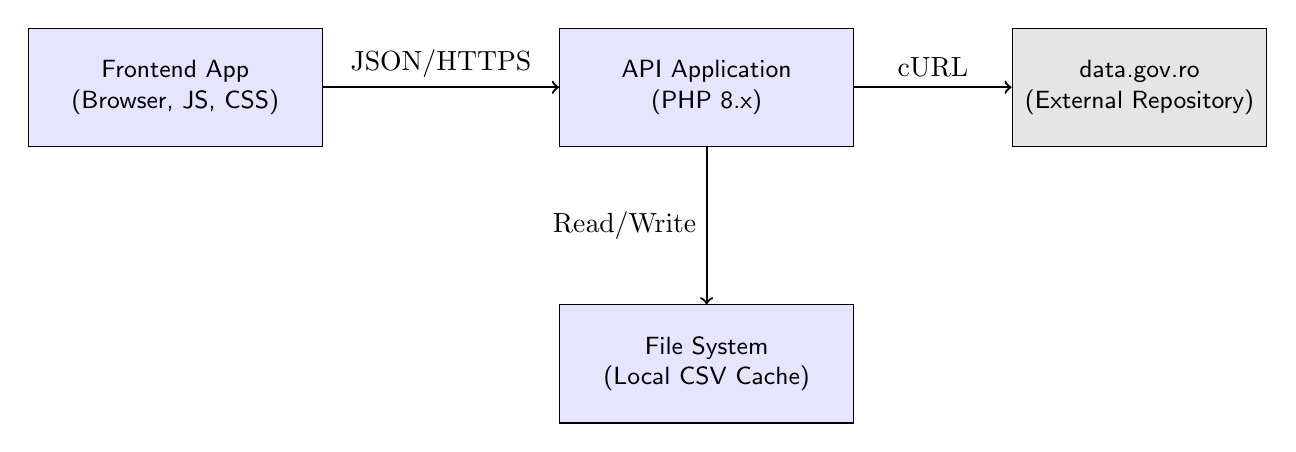
\begin{tikzpicture}[
    container/.style={rectangle, draw, fill=blue!10, text width=3.5cm, align=center, minimum height=1.5cm, font=\small\sffamily},
    external/.style={rectangle, draw, fill=gray!20, text width=3cm, align=center, minimum height=1.5cm, font=\small\sffamily}
]
    \node[container] (fe) {Frontend App\\(Browser, JS, CSS)};
    \node[container, right=3cm of fe] (api) {API Application\\(PHP 8.x)};
    \node[container, below=2cm of api] (cache) {File System\\(Local CSV Cache)};
    \node[external, right=2cm of api] (datagov) {data.gov.ro\\(External Repository)};

    \draw[->, thick] (fe) -- node[above] {JSON/HTTPS} (api);
    \draw[->, thick] (api) -- node[left] {Read/Write} (cache);
    \draw[->, thick] (api) -- node[above] {cURL} (datagov);
\end{tikzpicture}
\end{center}

\newpage
\subsection{Level 3: Component Diagram (Backend API)}
\begin{center}
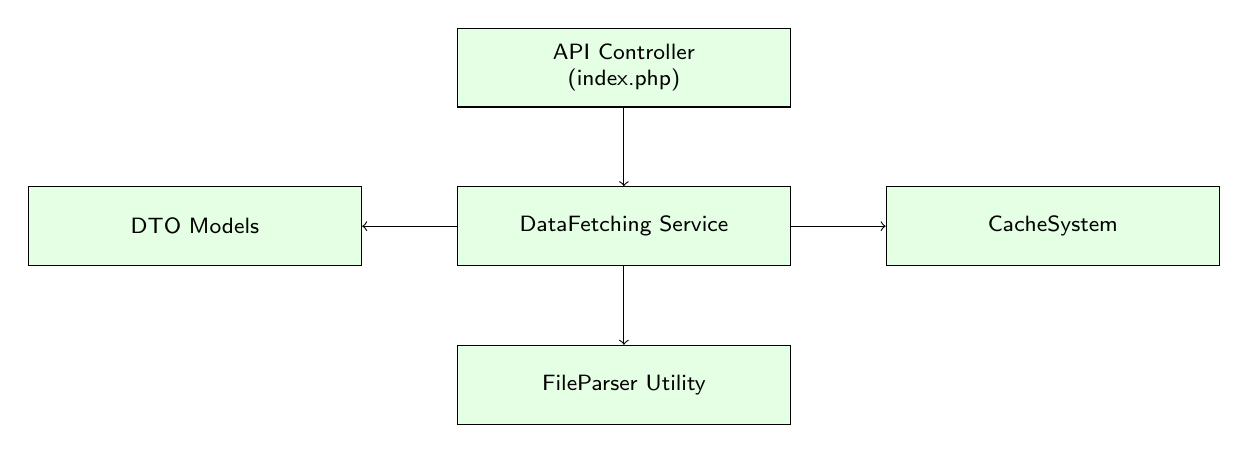
\begin{tikzpicture}[
    comp/.style={rectangle, draw, fill=green!10, text width=4cm, align=center, minimum height=1cm, font=\footnotesize\sffamily}
]
    \node[comp] (ctrl) {API Controller\\(index.php)};
    \node[comp, below=1cm of ctrl] (fetch) {DataFetching Service};
    \node[comp, below=1cm of fetch] (parser) {FileParser Utility};
    \node[comp, right=1.2cm of fetch] (cacheman) {CacheSystem};
    \node[comp, left=1.2cm of fetch] (models) {DTO Models};

    \draw[->] (ctrl) -- (fetch);
    \draw[->] (fetch) -- (parser);
    \draw[->] (fetch) -- (cacheman);
    \draw[->] (fetch) -- (models);
\end{tikzpicture}
\end{center}

\subsection{Level 4: Code Diagram (Class Structure Example)}
\begin{center}
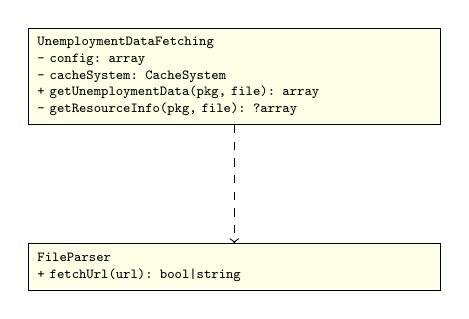
\begin{tikzpicture}[
    class/.style={rectangle, draw, fill=yellow!10, text width=5cm, font=\tiny\ttfamily}
]
    \node[class] (fetching) {
        \textbf{UnemploymentDataFetching}\\
        - config: array\\
        - cacheSystem: CacheSystem\\
        + getUnemploymentData(pkg, file): array\\
        - getResourceInfo(pkg, file): ?array
    };
    \node[class, below=1.5cm of fetching] (parser) {
        \textbf{FileParser}\\
        + fetchUrl(url): bool|string
    };
    \draw[->, dashed] (fetching) -- (parser);
\end{tikzpicture}
\end{center}

\newpage
\section{Arhitectura Sistemului}

Aplicația este construită pe un model \textbf{Decoupled Front-to-Back}, utilizând containere Docker pentru a asigura un mediu de rulare izolat, predictibil și ușor de scalat.

\subsection{Infrastructură: Dockerization}
Sistemul este orchestrat prin \texttt{docker-compose} și este compus din două servicii principale:
\begin{itemize}
    \item \textbf{Serviciul API}: Un container PHP-FPM/Apache care rulează nucleul logic de preluare și procesare a datelor. Acesta nu este expus direct utilizatorului final, comunicând doar în rețeaua internă Docker.
    \item \textbf{Serviciul Frontend}: Un container Apache care servește fișierele statice (HTML, CSS, JS) și include un script \texttt{api-proxy.php}.
\end{itemize}

\subsection{Comunicarea și Securitatea: API Proxy}
Pentru a evita problemele de \textbf{CORS (Cross-Origin Resource Sharing)} și pentru a menține API-ul într-o zonă securizată, comunicarea se face printr-un proxy:
\begin{enumerate}
    \item Frontend-ul (JS) trimite cereri către \texttt{api-proxy.php} aflat pe același host.
    \item Proxy-ul PHP utilizează \texttt{file\_get\_contents} pentru a comunica cu containerul \texttt{api} prin DNS-ul intern al Docker.
    \item Acest model permite ascunderea complexității infrastructurii și oferă un punct unic de control pentru cererile către datele externe.
\end{enumerate}

\subsection{Separarea Responsabilităților (Separation of Concerns)}
\begin{itemize}
    \item \textbf{Backend (Stateless)}: Se ocupă strict de fetching, parsare CSV, normalizare (curățarea diacriticelor corupte) și caching. Nu menține stări de sesiune ale utilizatorului.
    \item \textbf{Frontend (Stateful)}: Gestionează starea aplicației (\texttt{state} object), preferințele de filtrare ale utilizatorului și logica de randare a componentelor vizuale.
\end{itemize}

\section{Backend Documentation}

\subsection{API Reference}
Sistemul Backend oferă o interfață RESTful pentru consumul datelor statistice și gestionarea stării interne (cache).

\subsubsection{Endpoint: Fetch Data}
\begin{itemize}
    \item \textbf{Metodă}: \texttt{GET}
    \item \textbf{URL}: \texttt{/api/\{packageName\}/\{fileName\}}
    \item \textbf{Parametri}:
        \begin{itemize}
            \item \texttt{packageName}: ID-ul perioadei (ex: \texttt{mai2025}, \texttt{aprilie2024}).
            \item \texttt{fileName}: Tipul setului de date (\texttt{rata.csv}, \texttt{medii.csv}, \texttt{varste.csv}, \texttt{nivel-educatie.csv}).
        \end{itemize}
    \item \textbf{Răspuns}: JSON Array conținând obiectele DTO corespunzătoare setului cerut.
\end{itemize}

\subsubsection{Endpoint: Interactive Documentation (Swagger UI)}
\begin{itemize}
    \item \textbf{URL}: \texttt{/swagger/index.html}
    \item \textbf{Descriere}: Pagina statică ce expune documentația interactivă a API-ului. Încarcă biblioteca Swagger UI prin CDN și citește fișierul de specificație OpenAPI 3.0 din \texttt{/swagger/openapi.json}.
    \item \textbf{Funcționalitate}: Permite vizualizarea completă a endpoint-urilor, schemelor de date (DTOs) și executarea de cereri direct din browser utilizând butonul „Try it out”.
\end{itemize}

\subsubsection{Gestionarea Internă a Caching-ului}
API-ul implementează un sistem de cache automat pe fișiere (în directorul \texttt{cache/}) cu un timp de expirare (TTL) de 7 zile. Nu există endpoint-uri administrative publice expuse pentru cache; în schimb, sistemul se curăță singur automat la fiecare cerere primită prin intermediul metodei \texttt{CacheSystem::cleanExpired()} apelată în controller-ul principal (\texttt{index.php}).

\subsection{DTOs Structure (Models)}
Toate modelele folosesc proprietăți publice pentru o conversie facilă în JSON.

\subsubsection{UnemploymentDataBasic}
Mapat pe \texttt{rata.csv}.
\begin{itemize}
    \item \texttt{string \$county}: Numele județului.
    \item \texttt{int \$nrUnemployed}: Număr total șomeri.
    \item \texttt{int \$nrFemaleUnemployed}: Număr femei șomere.
    \item \texttt{int \$nrMaleUnemployed}: Număr bărbați șomeri.
    \item \texttt{int \$nrCompensatedUnemployed}: Șomeri indemnizați.
    \item \texttt{int \$nrNonCompensatedUnemployed}: Șomeri neindemnizați.
    \item \texttt{float \$unemploymentRate}: Rata șomajului (\%).
    \item \texttt{float \$femaleUnemploymentRate}: Rata șomajului în rândul femeilor (\%).
    \item \texttt{float \$maleUnemploymentRate}: Rata șomajului în rândul bărbaților (\%).
\end{itemize}

\subsubsection{UnemploymentDataPerAgeRange}
Mapat pe \texttt{varste.csv}.
\begin{itemize}
	\item \texttt{string \$county}: Județ.
	\item \texttt{int \$under25}: Număr șomeri sub vârsta de 25 ani. 
	\item \texttt{\$from25to29}: Număr șomeri între 25 și 29 de ani.
	\item \texttt{\$from30to39}: Număr șomeri între 30 și 39 de ani.
	\item \texttt{\$from40to49}: Număr șomeri între 40 și 49 de ani.
	\item \texttt{\$from50to59}: Număr șomeri între 50 și 59 de ani.
	\item \texttt{\$over50}: Număr șomeri peste 50 de ani.
\end{itemize}

\subsubsection{UnemploymentDataPerEducationLevel}
Mapat pe \texttt{nivel-educatie.csv}.
\begin{itemize}
	\item \texttt{string \$county}: Județ.
	\item \texttt{int \$noStudy}: Număr șomeri fără studii.
	\item \texttt{\$primaryStudy}: Număr șomeri cu studii primare. 
	\item \texttt{\$middleStudy}: Număr șomeri cu studii gimnaziale. 
	\item \texttt{\$highStudy}: Număr șomeri cu studii liceale. 
	\item \texttt{\$postHighStudy}: Număr șomeri cu studii postliceale. 
	\item \texttt{\$professionalStudy}: Număr șomeri cu studii profesionale. 
	\item \texttt{\$universityStudy}: Număr șomeri cu studii universitare.
\end{itemize}

\subsubsection{UnemploymentDataPerMedium}
Mapat pe \texttt{medii.csv}.
\begin{itemize}
    \item \texttt{string \$county}: Județ.
    \item \texttt{int \$totalUnemployed}: Total șomeri.
    \item \texttt{int \$totalFemaleUnemployed}: Femei șomere (total).
    \item \texttt{int \$totalMaleUnemployed}: Bărbați șomeri (total).
    \item \texttt{int \$totalUnemployedUrban}: Șomeri din mediu urban.
    \item \texttt{int \$totalFemaleUnemployedUrban}: Femei șomere din mediu urban.
    \item \texttt{int \$totalMaleUnemployedUrban}: Bărbați șomeri din mediu urban.
    \item \texttt{int \$totalUnemployedRural}: Șomeri din mediu rural.
    \item \texttt{int \$totalFemaleUnemployedRural}: Femei șomere din mediu rural.
    \item \texttt{int \$totalMaleUnemployedRural}: Bărbați șomeri din mediu rural.
\end{itemize}

\subsection{Caching and Transformation Strategy}
Sistemul de caching este implementat în clasa \texttt{CacheSystem} și are rolul de a optimiza performanța și de a asigura stabilitatea aplicației în cazul în care sursa externă este indisponibilă temporar.

\subsubsection{Mecanismul de Stocare}
Datele sunt stocate local în directorul \texttt{API/cache/} sub formă de fișiere CSV brute. Denumirea fișierelor urmează schema \texttt{\{package\_name\}\_\{file\_name\}}, asigurând unicitatea resurselor pentru fiecare lună și criteriu.

\subsubsection{Ciclul de Viață al Datelor (TTL)}
Aplicația implementează o politică de expirare automată a datelor:
\begin{itemize}
    \item \textbf{Durata de viață}: Fișierele sunt considerate valide timp de 7 zile (\texttt{CACHE\_LIFETIME = 604800} secunde).
    \item \textbf{Curățare Automată}: La fiecare cerere către \texttt{index.php}, sistemul scanează directorul de cache și șterge fișierele a căror dată de modificare (\texttt{filemtime}) este mai veche decât pragul setat.
    \item \textbf{Validare la Fetch}: În \texttt{UnemploymentDataFetching}, înainte de a iniția o cerere cURL, se verifică existența fișierului în cache. Dacă acesta lipsește, se descarcă de pe \texttt{data.gov.ro} și se salvează local prin metoda \texttt{CacheSystem::put()}.
\end{itemize}

\subsubsection{De ce convertim din CSV în JSON?}
\begin{enumerate}
    \item \textbf{Curățarea Datelor}: Fișierele sursă conțin adesea erori de encoding (ex: „Caraș-Severin” scris greșit). API-ul corectează aceste erori în timpul conversiei.
    \item \textbf{Performanță}: JSON-ul este mult mai rapid de parsat în Frontend decât un CSV brut, reducând timpul de blocare a thread-ului principal în browser.
    \item \textbf{Tipizarea și Normalizarea}: Conversia permite transformarea string-urilor din CSV în tipuri numerice (\texttt{int}/\texttt{float}) și eliminarea punctelor de separare a mii, asigurând calcule matematice corecte în grafice.
\end{enumerate}

\newpage
\section{Frontend Implementation}

\subsection{Mecanismul de Export}
Aplicația suportă cinci formate de export, fiecare folosind tehnici diferite de procesare a datelor.

\subsubsection{Export CSV (Date Tabelare)}
Sistemul generează fișiere CSV direct în browser:
\begin{itemize}
    \item \textbf{Separator}: Se folosește punct și virgulă (\texttt{;}) pentru compatibilitate cu setările regionale europene ale Microsoft Excel.
    \item \textbf{Diacritice}: Se prefixează conținutul cu un \textbf{Byte Order Mark (BOM)} (\texttt{\textbackslash uFEFF}) pentru a forța Excel să recunoască codarea UTF-8 și să afișeze corect caracterele românești.
\end{itemize}

\subsubsection{Export SVG (Vectorial)}
Deoarece Chart.js utilizează elementul \texttt{<canvas>} (bazat pe pixeli), exportul vectorial este realizat prin încapsulare:
\begin{enumerate}
    \item Se capturează canvas-ul curent ca un \textbf{DataURL (PNG)}.
    \item Se construiește un fișier XML SVG care conține un tag \texttt{<image>} cu sursa setată la DataURL-ul capturat.
    \item Această metodă permite integrarea graficului în documente vectoriale menținând rezoluția originală de randare.
\end{enumerate}

\subsubsection{Export PDF (Raport Complet)}
Folosește \textbf{jsPDF} și \textbf{jspdf-autotable} pentru un document multi-pagină:
\begin{itemize}
    \item \textbf{Fonturi Custom}: Încarcă fontul \textbf{Roboto} (Normal/Bold) asincron la runtime din directorul local pentru suportul diacriticelor, reducând dimensiunea inițială a paginii.
    \item \textbf{Integritate}: Spre deosebire de alte metode, PDF-ul re-parcurge întreg setul de date din \texttt{state.data} pentru a genera un tabel complet, ignorând limitările de paginare ale UI-ului.
    \item \textbf{Print Workflow}: Utilizează \texttt{pdf.autoPrint()} pentru a declanșa automat dialogul de sistem, facilitând utilizarea virtualizării precum \texttt{cups-pdf}.
\end{itemize}

\subsubsection{Export SQL (Migrare și Interoperabilitate)}
Aplicația permite transformarea datelor vizualizate în scripturi SQL gata de importat:
\begin{itemize}
    \item \textbf{Generare Dinamică}: Sistemul construiește instrucțiuni \texttt{CREATE TABLE} și \texttt{INSERT INTO} bazate pe structura DTO-ului curent.
    \item \textbf{Sanitizare}: Datele sunt curățate pentru a preveni erorile de sintaxă SQL (ex: escape pentru ghilimelele din numele județelor).
    \item \textbf{Cazul de utilizare}: Facilitează integrarea rapidă a datelor de la \textbf{data.gov.ro} în sisteme de management al bazelor de date (RDBMS) externe pentru analize complexe.
\end{itemize}

\subsubsection{Export JSON (Sursă Brută)}
Pentru dezvoltatori și analiști, aplicația oferă exportul stării curente în format JSON:
\begin{itemize}
    \item \textbf{Structură Fidelă}: Fișierul generat păstrează ierarhia obiectelor JavaScript din \texttt{state}, oferind acces la toate metadatele procesate de API.
    \item \textbf{Portabilitate}: Formatul JSON asigură cea mai mare compatibilitate cu alte limbaje de programare (Python, R, Java) pentru procesări ulterioare în fluxuri de Data Science.
\end{itemize}

\subsection{Harta Interactivă (Leaflet)}
Afișarea hărții se bazează pe biblioteca \textbf{Leaflet}.
\begin{enumerate}
    \item \textbf{GeoJSON}: Granitele județelor sunt încărcate dintr-un fișier extern GeoJSON.
    \item \textbf{Colorare}: Funcția \texttt{getColor(rate)} mapează rata șomajului pe o paletă de culori de la verde la roșu.
    \item \textbf{Normalizare}: Deoarece numele județelor în GeoJSON diferă de cele din sursa oficială, se folosește o funcție de normalizare a string-urilor.
\end{enumerate}

\subsection{Randarea Graficelor (Chart.js)}
Graficele sunt desenate dinamic în elemente \texttt{<canvas>}.
\begin{itemize}
    \item \textbf{Bar Chart}: Folosit pentru evoluția pe județe. Suportă modul „Stacked” pentru criterii multiple și modul „Comparison” pentru două perioade.
    \item \textbf{Donut Chart}: Folosit pentru distribuția procentuală. Centrul graficului afișează automat procentul celei mai mari categorii.
\end{itemize}

\end{document}
